\newpage
\chapter{程式講解}
\section{設定句柄變數}
\begin{figure}[hbt!]
\begin{center}
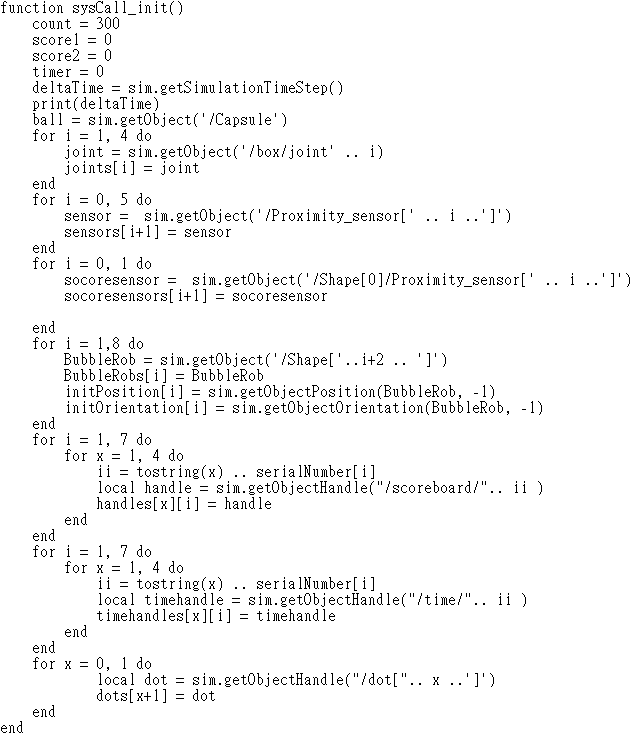
\includegraphics[width=12cm]{1}
\caption{\Large 設定句柄變數}\label{設定句柄變數}
\end{center}
\end{figure} 
這段程式碼,如(圖.\ref{設定句柄變數}),功能性及註解,如(圖.\ref{設定句柄變數註解})\
\begin{figure}[hhtbp!]
\begin{center}
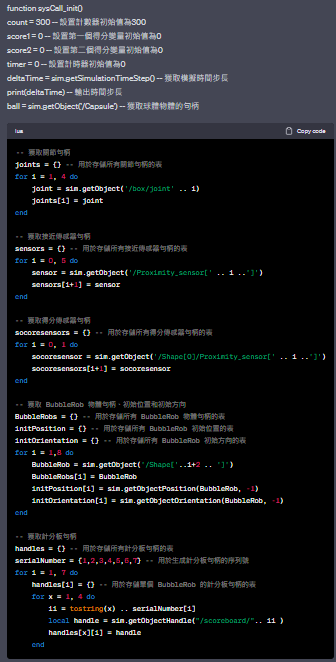
\includegraphics[width=12cm]{1解說}
\caption{\Large 設定句柄變數註解}\label{設定句柄變數註解}
\end{center}
\end{figure}
\
\newpage
\
\section{回復記分板顏色}
\begin{figure}[htbp!]
\begin{center}
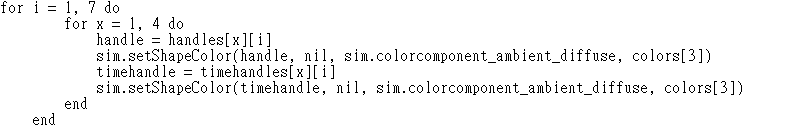
\includegraphics[width=12cm]{2}
\caption{\Large 回復記分板顏色}\label{回復記分板顏色}
\end{center}
\end{figure} 
\
這段程式碼,如(圖.\ref{回復記分板顏色}),四、六行註解為設置計分板形狀的顏色為 color3。
\section{產生隨機座標}
\begin{figure}[htbp!]
\begin{center}
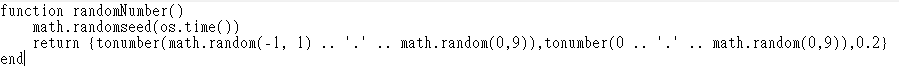
\includegraphics[width=12cm]{3}
\caption{\Large 產生隨機座標}\label{產生隨機座標}
\end{center}
\end{figure} 
\
這段程式碼,如(圖.\ref{產生隨機座標}),第二行註解為使用當前時間作為隨機亂數。
\section{設定記分板顏色}
\begin{figure}[htbp!]
\begin{center}
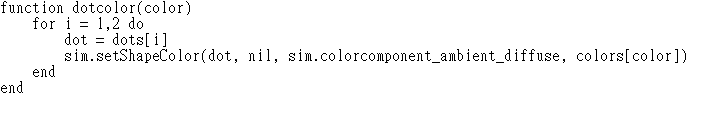
\includegraphics[width=12cm]{4}
\caption{\Large 設定記分板顏色}\label{設定記分板顏色}
\end{center}
\end{figure} 
\
這個函式,如(圖.\ref{設定記分板顏色})用於設置兩個點的顏色。它接受一個參數 color,用於指定要設置的顏色。在函式內部,使用 sim.setShapeColor 函式將顏色應用到每個點的形狀上,使用 colors[color] 來獲取指定的顏色。
\section{分解剩餘時間數字}
\begin{figure}[htbp!]
\begin{center}
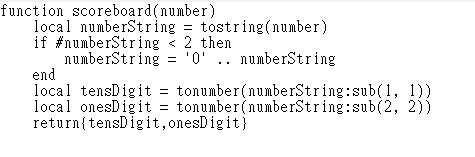
\includegraphics[width=12cm]{5}
\caption{\Large 分解剩餘時間數字}\label{分解剩餘時間數字}
\end{center}
\end{figure} 
\
這個函式,如(圖.\ref{分解剩餘時間數字})用於將數字轉換為計分板的十位數和個位數。它接受一個參數 number,代表要轉換的數字。首先,將數字轉換為字符串 numberString。如果 numberString 的長度小於 2,則在前面添加一個 '0',確保有兩位數字。然後,使用 tonumber 和 string.sub 函式提取十位數和個位數,分別存儲在 tensDigit 和 onesDigit 中。最後,返回一個包含十位數和個位數的數組。
\section{感測得分並修改記分板}
\begin{figure}[htbp!]
\begin{center}
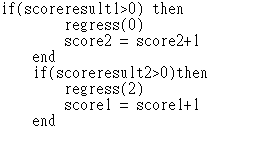
\includegraphics[width=12cm]{6}
\caption{\Large 感測得分並修改記分板}\label{感測得分並修改記分板}
\end{center}
\end{figure} 
\
這個函式,如(圖.\ref{感測得分並修改記分板})包含兩個條件語句。第一個條件語句檢查 scoreresult1 是否大於 0,如果是,則執行 regress(0) 函式並將 score2 加一。第二個條件語句檢查 scoreresult2 是否大於 0,如果是,則執行 regress2)函式並將 score1 加一。
\newpage
\section{將即時分數顯示在計分板}
\begin{figure}[htbp!]
\begin{center}
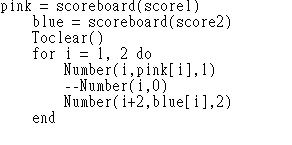
\includegraphics[width=12cm]{7}
\caption{\Large 將即時分數顯示在計分板}\label{將即時分數顯示在計分板}
\end{center}
\end{figure} 
\
這個函式,如(圖.\ref{將即時分數顯示在計分板})首先將 score1 轉換為十位數和個位數,並將結果存儲在 pink 中。然後將 score2 轉換為十位數和個位數,並將結果存儲在 blue 中。接下來調用 Toclear 函式。\\
接下來的迴圈對於 i 等於 1 到 2,進行以下操作:\\
使用 Number i, pink i , 1 將 pink 中的十位數或個位數設置到數字顯示器中,並設置為顏色 1。\\
使用 Number i加2, blue i, 2 將 blue 中的十位數或個位數設置到數字顯示器中,並設置為顏色 2。\\
\section{時間到則停止遊戲}
\begin{figure}[htbp!]
\begin{center}
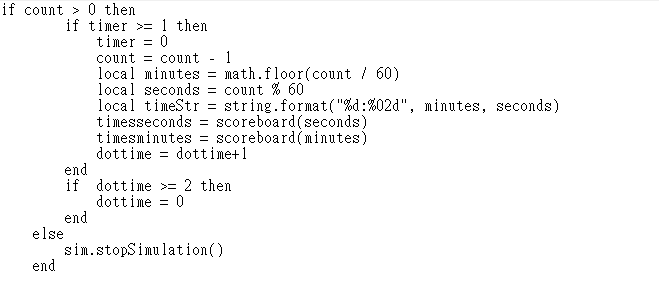
\includegraphics[width=12cm]{8}
\caption{\Large 時間到則停止遊戲}\label{時間到則停止遊戲}
\end{center}
\end{figure} 
\
這個函式,如(圖.\ref{時間到則停止遊戲})包含一個條件語句。首先檢查 count 是否大於 0,如果是,則執行以下操作:\\
檢查 timer 是否大於等於 1,如果是,則將 timer 重置為 0,並將 count 減一。\\
根據 count 計算出分鐘數和秒數,並使用 string.format 函式將其格式化為 分鐘:秒 的字符串形式。\\
將秒數和分鐘數分別轉換為十位數和個位數,並將結果分別存儲在 timesseconds 和 timesminutes 中。
將 dottime 加一。\\
接下來,檢查 dottime 是否大於等於 2,如果是,則將 dottime 重置為 0。\\
如果 count 小於等於 0,則執行 sim.stopSimulation函式停止仿真。\\
\section{回復記分板顏色}
\begin{figure}[htbp!]
\begin{center}
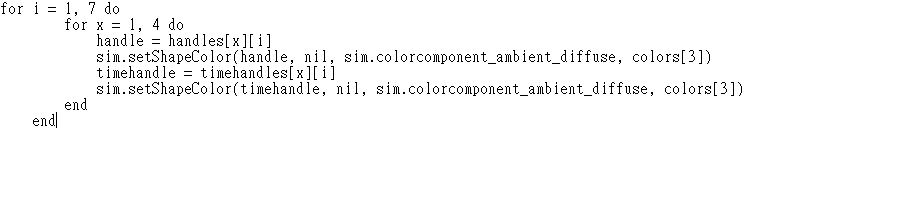
\includegraphics[width=12cm]{9}
\caption{\Large 回復記分板顏色}\label{回復記分板顏色}
\end{center}
\end{figure} 
\
這個函式,如(圖.\ref{回復記分板顏色})使用兩個嵌套的迴圈。外層迴圈遍歷 i 從 1 到 7 的值,內層迴圈遍歷 x 從 1 到 4 的值。\\
對於每一個 i 和 x 的組合,執行以下操作:\\
從 handles 中獲取 handle 的值。
使用 sim.setShapeColor 函式將 handle 的形狀顏色設置為 colors3。
從 timehandles 中獲取 timehandle 的值。
使用 sim.setShapeColor 函式將 timehandle 的形狀顏色設置為 colors3。
換句話說,這段代碼將遍歷一個二維數組 handles 和 timehandles,並將相應的形狀顏色設置為 colors3。\\
